%\label{Maze}
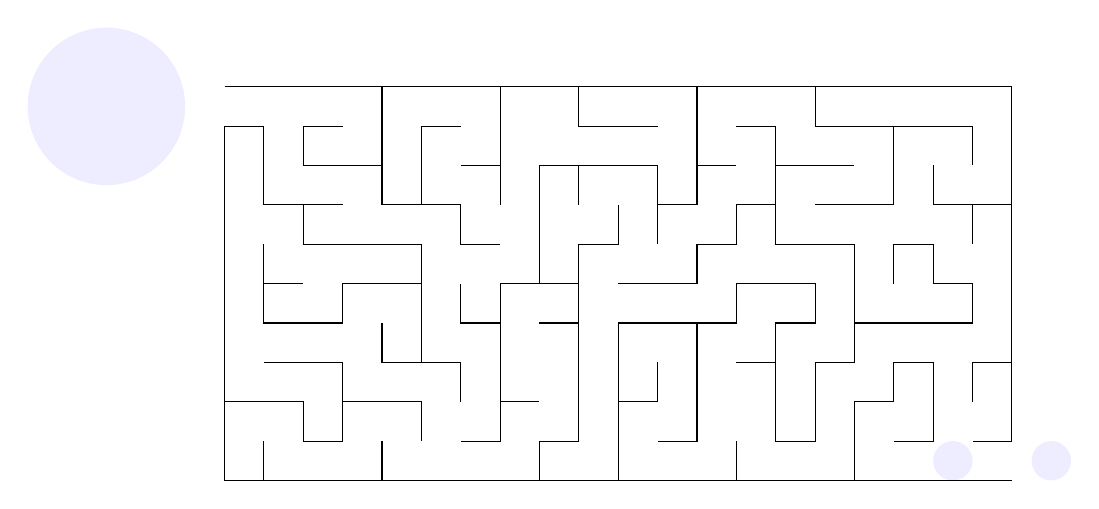
\begin{tikzpicture}[scale=0.5]
% Water
\fill[blue!7] (-3,9.5) circle (2);
\fill[blue!7] (18.5,0.5) circle (0.5);
\fill[blue!7] (21,0.5) circle (0.5);

% outer lines
\draw (0,10) -| (20,1) -- +(-1,0);
\draw (20,0) -| (0,9) -| (1,7) -- (3,7);
\draw (2,7) |- (5,6) |- (6,3) -- (6,2);
\draw (5,3) -| (4,4);
\draw (5,5) -| (3,4) -| (1,6); \draw (1,5) -- (2,5);

% bottom row
\draw (0,2) -| (2,1) -| (3,3) -- (1,3); \draw (3,2) -| (5,1);
\draw (1,0) -- (1,1);
\draw (4,0) -- (4,1);
\draw (8,0) |- (9,1) |- (10,6) -- (10,7); \draw (8,4) -- (9,4); \draw (8,5) -- (9,5);

\draw (10,0) |- (13,4) |- (15,5) |- (14,4) |- (15,1) |- (16,3) |- (14,6) |- (13,9);
\draw (10, 2) -| (11,3); \draw (12,4) |- (11,1); \draw (13,3) -- (14,3);
\draw (16,4) -| (19,5) -| (18,6) -| (17,5);
\draw (14,7) -| (13,6) -| (12,5) -- (10,5); \draw (14,8) -- (16,8);

\draw (13,0) -- (13,1);
\draw (16,0) |- (17,2) |- (18,3) |- (17,1);
\draw (20,3) -| (19,2);

% top row
\draw (4,10) |- (6,7) |- (7,6); \draw (4,8) -- (2,8) |- (3,9); \draw (5,7) |- (6,9);
\draw (7,10) -- (7,7); \draw (7,8) -- (6,8);
\draw (9,10) |- (11,9);
\draw (12,10) |- (11,7); \draw (11,6) |- (8,8) |- (7,5) |- (6,1);
\draw (12,8) -- (13,8); \draw (9,8) -- (9,7); \draw (7,4) -| (6,5); \draw (7,2) -- (8,2);
\draw (15,10) |- (19,9) -- (19,8); \draw (17,9) |- (15,7);
\draw (20,7) -| (18,8); \draw (19,7) -- (19,6);
\end{tikzpicture}

\begin{figure}[h]\label{MazeStain}
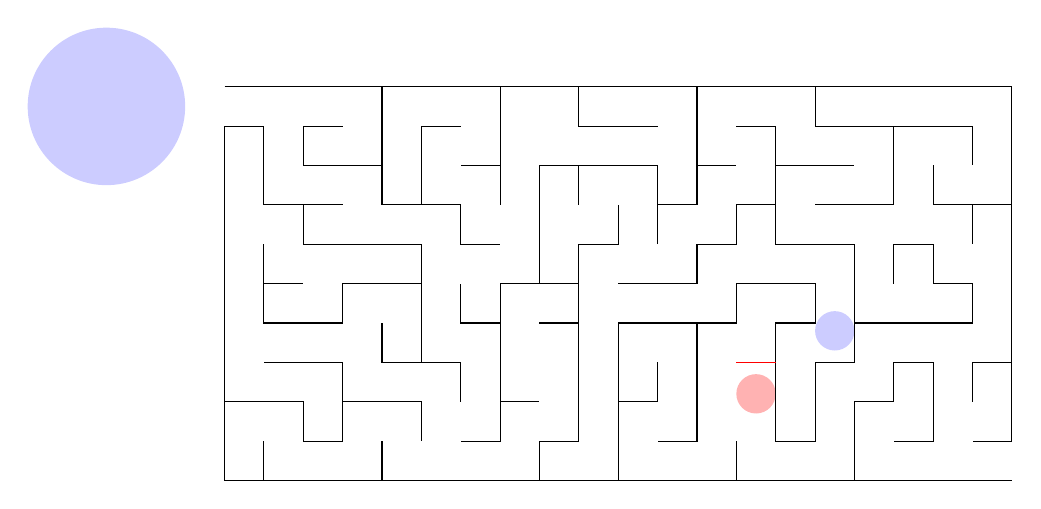
\begin{tikzpicture}[scale=0.5]
% Water
\fill[blue!20] (-3,9.5) circle (2);
%\fill[blue!20] (18.5,0.5) circle (0.5);
%\fill[blue!20] (21,0.5) circle (0.5);
\fill[red!30] (13.5,2.2) circle (0.5);
\fill[blue!20] (15.5,3.8) circle (0.5);

% outer lines
\draw (0,10) -| (20,1) -- +(-1,0);
\draw (20,0) -| (0,9) -| (1,7) -- (3,7);
\draw (2,7) |- (5,6) |- (6,3) -- (6,2);
\draw (5,3) -| (4,4);
\draw (5,5) -| (3,4) -| (1,6); \draw (1,5) -- (2,5);

% bottom row
\draw (0,2) -| (2,1) -| (3,3) -- (1,3); \draw (3,2) -| (5,1);
\draw (1,0) -- (1,1);
\draw (4,0) -- (4,1);
\draw (8,0) |- (9,1) |- (10,6) -- (10,7); \draw (8,4) -- (9,4); \draw (8,5) -- (9,5);

\draw (10,0) |- (13,4) |- (15,5) |- (14,4) |- (15,1) |- (16,3) |- (14,6) |- (13,9);
\draw (10, 2) -| (11,3); \draw (12,4) |- (11,1);
 \draw[red] (13,3) -- (14,3);
\draw (16,4) -| (19,5) -| (18,6) -| (17,5);
\draw (14,7) -| (13,6) -| (12,5) -- (10,5); \draw (14,8) -- (16,8);

\draw (13,0) -- (13,1);
\draw (16,0) |- (17,2) |- (18,3) |- (17,1);
\draw (20,3) -| (19,2);

% top row
\draw (4,10) |- (6,7) |- (7,6); \draw (4,8) -- (2,8) |- (3,9); \draw (5,7) |- (6,9);
\draw (7,10) -- (7,7); \draw (7,8) -- (6,8);
\draw (9,10) |- (11,9);
\draw (12,10) |- (11,7); \draw (11,6) |- (8,8) |- (7,5) |- (6,1);
\draw (12,8) -- (13,8); \draw (9,8) -- (9,7); \draw (7,4) -| (6,5); \draw (7,2) -- (8,2);
\draw (15,10) |- (19,9) -- (19,8); \draw (17,9) |- (15,7);
\draw (20,7) -| (18,8); \draw (19,7) -- (19,6);
\end{tikzpicture}
\caption{Maze with stained water drops}
\end{figure}

\label{wifiRoom}
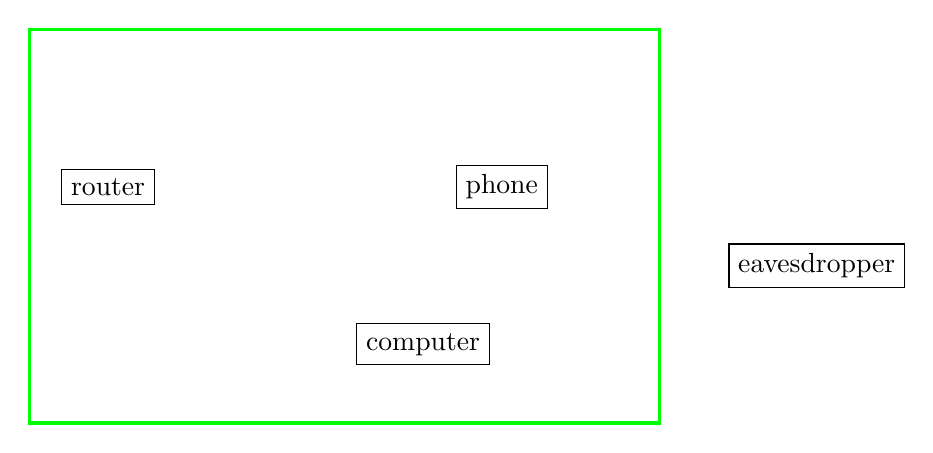
\begin{tikzpicture}
\draw[green, very thick] (0,0) rectangle (8,5);
\draw (1,3) node(router) [rectangle, draw] {router};
\draw (6,3) node(phone) [rectangle, draw] {phone};
\draw (5,1) node(computer) [rectangle, draw] {computer};
\draw (10,2) node(eavesdropper) [rectangle, draw] {eavesdropper};
\end{tikzpicture}

%\label{Room-WiFi}
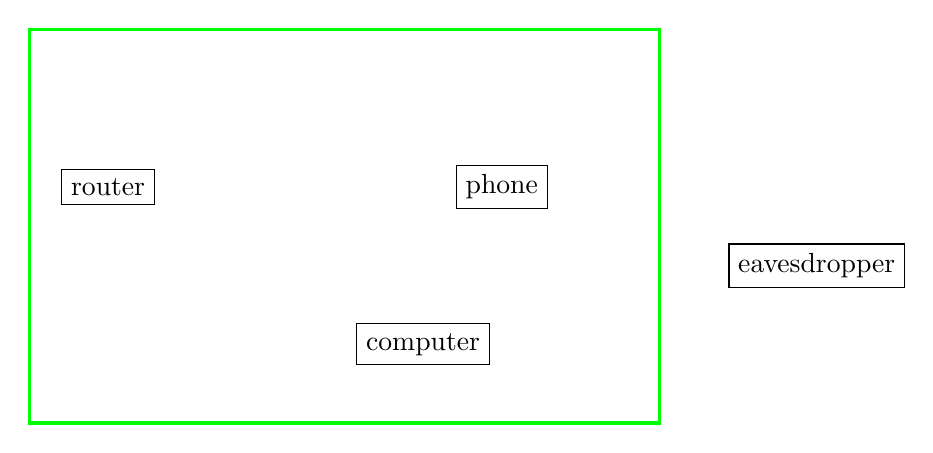
\begin{tikzpicture}
\draw[green, very thick] (0,0) rectangle (8,5);
\draw (1,3) node(router) [rectangle, draw] {router};
\draw (6,3) node(phone) [rectangle, draw] {phone};
\draw (5,1) node(computer) [rectangle, draw] {computer};
\draw (10,2) node(eavesdropper) [rectangle, draw] {eavesdropper};
\end{tikzpicture}

%\label{AirDrop}
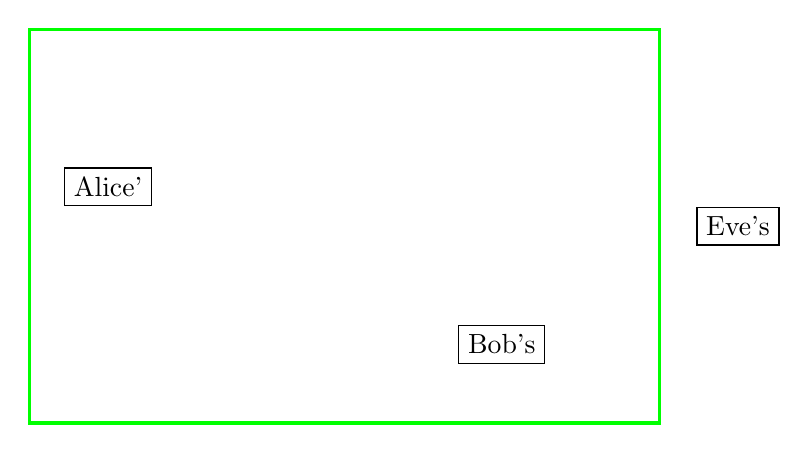
\begin{tikzpicture}
\draw[green, very thick] (0,0) rectangle (8,5);
\draw (1,3) node(router) [rectangle, draw] {Alice'};
\draw (6,1) node(computer) [rectangle, draw] {Bob's};
\draw (9,2.5) node(eavesdropper) [rectangle, draw] {Eve's};
\end{tikzpicture}

%\label{String}
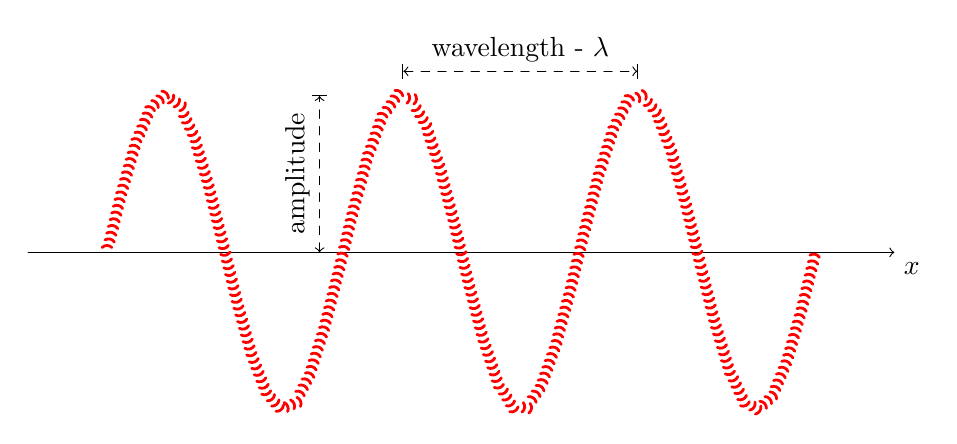
\begin{tikzpicture}[line join=round, line cap=round]

  % draw coordinate
  \draw[->] (-1,0) -- (10,0) node[pos=1.02,below] {$x$};
 % \draw[->] (0, -1) -- (0,2);
  % Rope properties
  \def\length{9}  % Length of the rope
  \def\thickness{1}  % Thickness of the rope
  \def\waveAmplitude{2}  % Amplitude of the wave
  \def\waveLength{3}  % Wavelength
  \def\segments{50}  % Number of segments
  
  % Draw the rope
  \draw[decorate, decoration={waves, segment length=2.5}, line width=\thickness, red]
    (0,0) -- plot[domain=0:\length, samples=\segments]
    (\x, {\waveAmplitude*sin(\x*(360/\waveLength))}) -- (\length,0);

    % label
    %\draw[red, fill] (3.75,2) circle(0.05cm);
    %\draw[red, fill] (6.75,2) circle(0.05cm);
    %\draw[dashed] (2,2) -- (3.75,2);
    \draw[<->|, dashed] (2.7,0) -- (2.7,2) node[pos=0.5, rotate = 90, above] {amplitude};
    \draw[|<->|, dashed] (3.75,2.3) -- (6.75,2.3) node[pos=0.5, above] {wavelength - $\lambda$};

\end{tikzpicture}

%\label{Wave}
\begin{tikzpicture}[scale=1.2]
    \draw[->] (-3.8,0) -- (3.9, 0)  node[pos=1.02,below] {$t$};
    \draw[->] (0,-3.5) -- (0,3.5);
    \draw[dotted, red] (-3.5,0) sin (-2.5,3) cos (-1.5,0) sin (-0.5,-3) cos (0.5,0) sin (1.5,3) cos (2.5,0) sin (3.5,-3);
    \draw[red, fill] (-2.5,3) circle(0.05cm);
    \draw[red, fill] (1.5,3) circle(0.05cm);
    \draw[dashed] (-2.5,0) -- (-2.5,3) node[pos=0.5, rotate = 90, above] {amplitude};
    \draw[dashed] (-2.5,3) -- (1.5,3) node[pos=0.3, above] {period - $T$};
    \draw[red, fill] (0.5,0) circle(0.05cm);
    \draw[dashed] (0.25,-0.1) -- (1,-2) node[below] {phase};
\end{tikzpicture}

%\label{PM}
\begin{tikzpicture}
    \draw[->] (-3.5,0) -- (3.5, 0);
    \draw[->] (0,-3.5) -- (0,3.5);
    \draw[dotted, red] (0,0) circle(3cm);
    \draw[red, fill] (30:3) circle(0.05cm);
    \draw[dashed] (1,0) arc (0:30:1) node[right, pos=0.6]{$\varphi$ - phase};
    \draw[dashed] (30:0.1) -- (30:2.9) node[pos=0.5, rotate = 30, above] {amplitude};
\end{tikzpicture}

%\label{QPSK}
\begin{tikzpicture}
    \draw[->] (-3.5,0) -- (3.5, 0);
    \draw[->] (0,-3.5) -- (0,3.5);
    \draw[dotted, red] (0,0) circle(3cm);
    \draw[red, fill] (3,0) circle(0.05cm) node[below right] {0};
    \draw[red, fill] (0,3) circle(0.05cm) node[above right] {1};
    \draw[red, fill] (-3,0) circle(0.05cm) node[above left] {10};
    \draw[red, fill] (0,-3) circle(0.05cm) node[below left] {11};
\end{tikzpicture}
%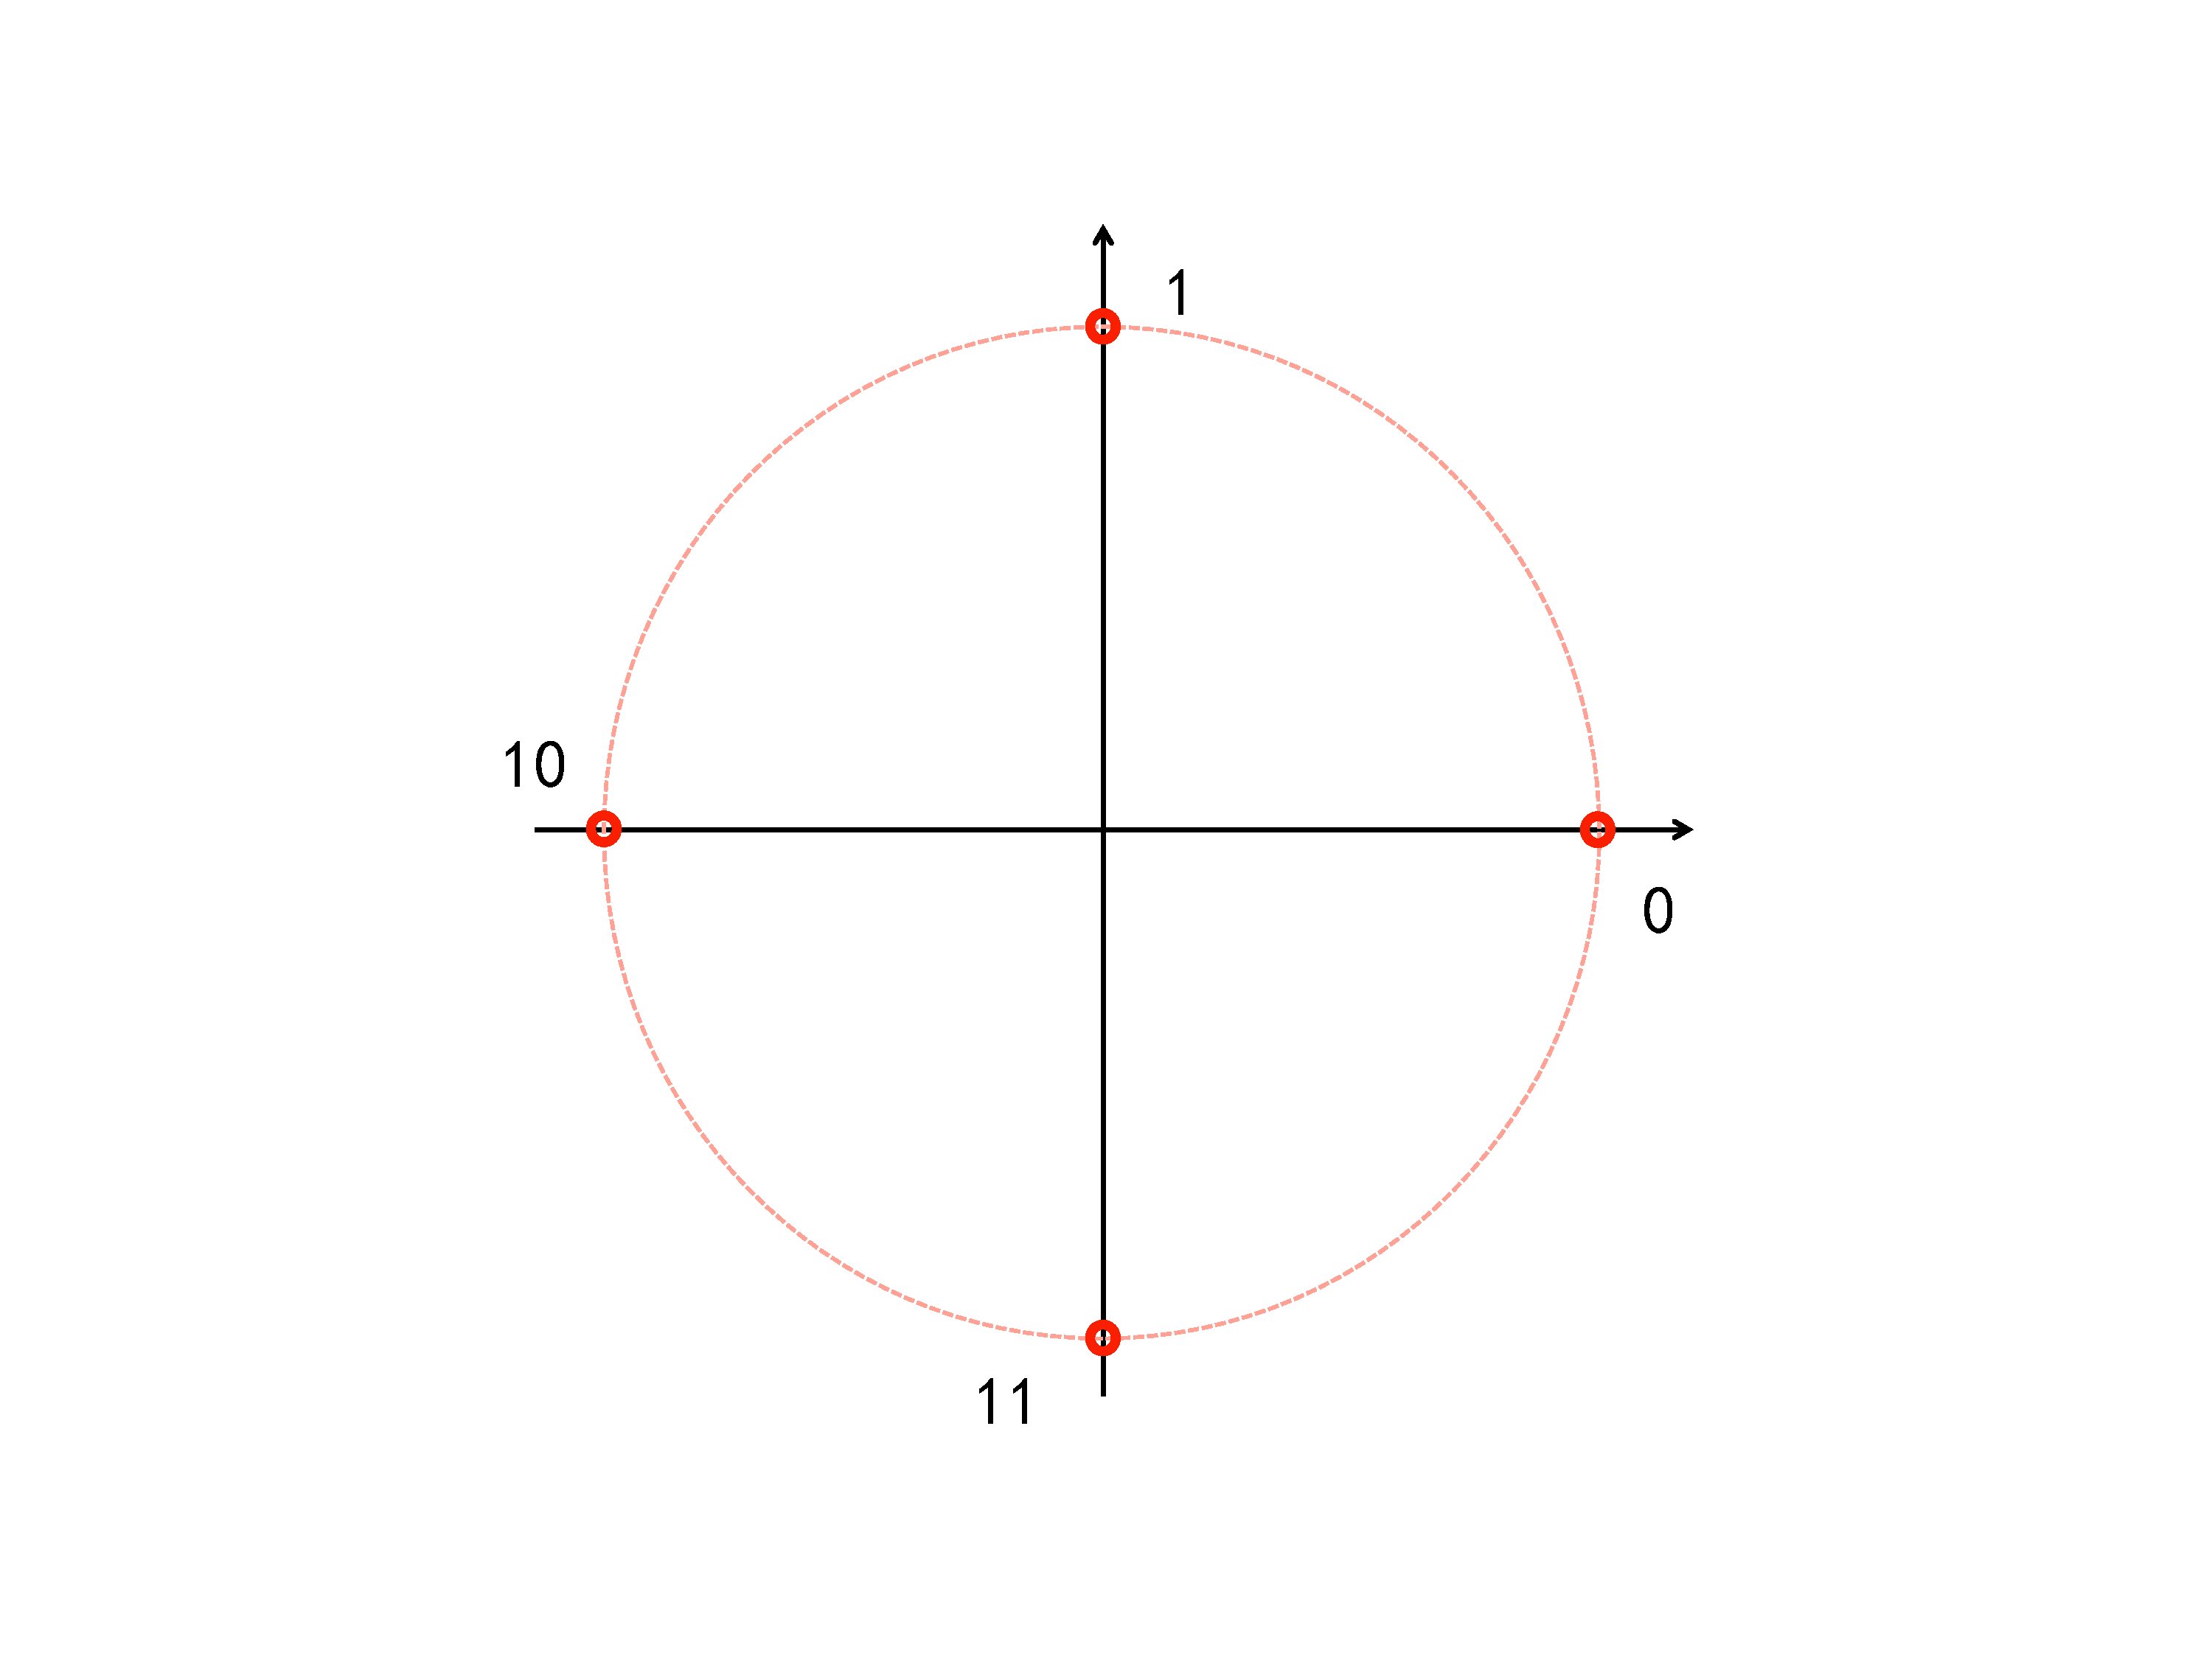
\includegraphics[width=6cm]{pic/4qpsk.pdf}
%\caption{QPSK constellation diagram}

%\label{sQPSK}
\begin{tikzpicture}
    \draw[->] (-3.5,0) -- (3.5, 0);
    \draw[->] (0,-3.5) -- (0,3.5);
    \draw[dashed] (2.5,2.5) -- (0, 0);
    \draw[dotted, red] (0,0) circle(3cm);
    \draw[red, fill] (2.12,2.12) circle(0.05cm) node[right] {11};
    \draw[red, fill] (-2.12,2.12) circle(0.05cm) node[above] {01};
    \draw[red, fill] (2.12,-2.12) circle(0.05cm) node[below] {10};
    \draw[red, fill] (-2.12,-2.12) circle(0.05cm) node[left] {00};
    \draw[dashed] (1,0) arc (0:45:1) node[right, pos=0.6]{$\varphi=45\circ$};
\end{tikzpicture}

\label{Modulator}
\begin{tikzpicture}
    \path %(-5,0) node[anchor=east] (start) {Wave} 
    (-3.5,-0.8) node[circle, draw=black] (lo) {$\sim$}
    (-3.5,0.8) node[Gate] (p90) {$90^\circ$}
    (0,2) node[Gate, text width=30] (tm) {$0/180^\circ$}
    (0,-2) node[Gate, text width=30] (bm) {$0/180^\circ$}
    (2,0) node[circle, draw=black] (add) {$\Sigma$}
     (3,0) node[anchor=west] (output) {wave output};
    \draw (lo.east) node[anchor=west] {carrier wave generator};
    \draw (add.west) node[anchor=east] {signal wave mixer};
    \draw (p90.east) node[anchor=west] {phase shifter};
    \draw (tm.north east) node[anchor=west] {controlled phase shifter};
    \draw (bm.south east) node[anchor=west] {controlled phase shifter};
    \draw (lo) -- (p90) |- (tm) -| (add);
    \draw (lo) |- (bm) -| (add);
    \draw (add) -- (output);
    \path (-2,3) node[anchor=east] (even) {data input - even bits}
    (-2,-3) node [anchor=east] (odd) {data input - odd bits};
    \draw[double] (even) -| (tm);
    \draw[double] (odd) -| (bm);
\end{tikzpicture}

\begin{figure}[ht]\label{modulator1}
\label{modulator1}
\begin{tikzpicture}
    \path
    (-2,-1) node[circle, draw=black] (lo) {$\sim$}
    (0,-1) node[circle, draw=black] (splitter) {$\prec$}
    (0,1) node[Gate] (p90) {$90^\circ$}
    (0,3) node[Gate] (ta) {$180^\circ$}
    (0,-3) node[Gate] (ba) {$180^\circ$}
    (3,0) node[circle, draw=black] (coupler) {$\succ$}
     (4,0) node[text width=60, align=center, anchor=west] (output) {signal wave output};
    \path (-2,3) node[text width=50, align=left, anchor=east] (even) {data input - even bits}
    (-2,-3) node [text width=50, align=left, anchor=east] (odd) {data input - odd bits};

    \draw (lo.north) node[text width=80, align=center, anchor=east] {wave generator};
    \draw (splitter.south east) node[text width=40, align=center, anchor=west] {50:50 splitter};
    \draw (p90.north west) node[text width=40, align=center, anchor=east] {phase shifter};
    \draw (ta.north) node[anchor=south] {controlled phase shifter};
    \draw (ba.south) node[anchor=north] {controlled phase shifter};
    \draw (coupler.north west) node[text width=40, align=center, anchor=east] {coupler};
    \draw (coupler) -- (output);
    \draw (ba) -- (splitter) -- (p90) -- (ta) -| (coupler) |- (ba);
    \draw (lo) -- (splitter);
    \draw[double] (even) -- (ta);
    \draw[double] (odd) -- (ba);
\end{tikzpicture}

\caption{QPSK modulator circuit}
\end{figure}

%\label{Demodulator}
\begin{tikzpicture}[scale=0.8]
    \path
    (0,-0.8) node[circle, draw=black] (lo) {$\sim$}
    (0,0.8) node[Gate] (p90) {$90^\circ$}
    (0,2) node[circle, draw=black] (ta) {X}
    (0,-2) node[circle, draw=black] (ba) {X}
    (2,2) node[Gate] (tm) {$\int$}
    (2,-2) node[Gate] (bm) {$\int$}
    (-3,0) node[circle, draw=black] (split) {$\prec$}
     (-4,0) node[text width=40, align=center, anchor=east] (input) {signal wave input};
    \path (3.5,2) node[text width=60, align=left, anchor=west] (even) {data output - even bits}
    (3.5,-2) node [text width=60, align=left, anchor=west] (odd) {data output - odd bits};

    \draw (lo.east) node[text width=50, align=center, anchor=west] {local wave generator};
    \draw (p90.east) node[text width=40, align=center, anchor=west] {phase shifter};
    \draw (tm.north) node[anchor=south] {detector};
    \draw (bm.south) node[anchor=north] {detector};
    \draw (ta.north) node[anchor=south] {mixer};
    \draw (ba.south) node[anchor=north] {mixer};
    \draw (bm) -- (ba) -- (lo) -- (p90) -- (ta) -- (tm);
    \draw[double] (even) -- (tm);
    \draw[double] (odd) -- (bm);

    \draw (ba) -| (split)  |- (ta);
    \draw (split.south east) node[text width=40, align=center, anchor=west] {50:50 splitter};
    \draw (split) -- (input);    
\end{tikzpicture}

\tdplotsetmaincoords{60}{110}

\begin{figure}
\begin{tikzpicture}[tdplot_main_coords, scale=1.5]

% Define colors
\definecolor{electriccolor}{RGB}{255,0,0}
\definecolor{magneticcolor}{RGB}{0,0,255}

% Draw coordinate axes
\draw[-latex] (0,0,0) -- (2,0,0) node[right] {$z$};
\draw[-latex] (0,0,0) -- (0,6,0) node[right] {$x$};
\draw[-latex] (0,0,0) -- (0,0,2) node[right] {$y$};

% Draw propagation arrow
\draw[-latex,thick] (0, 5.5,0) -- (0,6,0) node[below] {Propagation};

% Draw electric field wave (red)
\draw[electriccolor,thick,variable=\t,domain=-0.2:5.2,samples=54] 
  plot ({0,\t, sin(\t*180)*0.8});

% Draw magnetic field wave (blue)
\draw[magneticcolor,thick,variable=\t,domain=-0.3:5.2,samples=55] 
  plot ({sin(\t*180)*0.6},\t,0);

% Add labels for E and B fields
\node[electriccolor] at (0, 0.4,1.15) {$E$};
\node[magneticcolor] at (0.9, 0.43,0) {$B$};

% Add field direction indicators
\foreach \x in {0.5} {
  \draw[-latex,electriccolor] (0,\x,0) -- (0,\x,{sin(\x*180)});
  \draw[-latex,magneticcolor] (0,\x,0) -- ({sin(\x*180)*0.6},\x,0);
}
\end{tikzpicture}
\caption{Electric and Magnetic Fields of a Linearly Polarized Light}
\end{figure}

%\label{Modulator-DP-QPSK}
\begin{tikzpicture}
    \path
    (-2,-1) node[circle, draw=black] (lo) {$\sim$}
    (0,-1) node[circle, draw=black] (splitter) {$\prec$}
    (0,1) node[Gate] (p90) {$90^\circ$}
    (0,3) node[Gate] (ta) {$M$}
    (0,-3) node[Gate] (ba) {$M$}
    (3,0) node[circle, draw=black] (coupler) {$\succ$}
     (4,0) node[text width=60, align=center, anchor=west] (output) {signal wave output};
    \path (-2,3) node[text width=50, align=left, anchor=east] (even) {2-bit data input}
    (-2,-3) node [text width=50, align=left, anchor=east] (odd) {2-bit data input};

    \draw (lo.north) node[text width=80, align=center, anchor=east] {wave generator};
    \draw (splitter.south east) node[text width=40, align=center, anchor=west] {50:50 splitter};
    \draw (p90.east) node[text width=40, align=center, anchor=west] {polarizer};
    \draw (ta.north east) node[anchor=south] {QPSK modulator};
    \draw (coupler.west) node[text width=40, align=center, anchor=east] {coupler};
    \draw (coupler) -- (output);
    \draw (ba) -- (splitter) -- (p90) -- (ta) -| (coupler) |- (ba);
    \draw (lo) -- (splitter);
    \draw[double] (even) -- (ta);
    \draw[double] (odd) -- (ba);
\end{tikzpicture}

%\label{Demodulator-DP-QPSK}
\begin{tikzpicture}[scale=1]
    \path
    (-3,0) node[text width=40, align=center, anchor=east] (input) {signal wave input}
    (-2,0) node[circle, draw=black] (split) {$\prec$}
    (0,2) node[Gate] (tsp) {$D$}
    (0,-2) node[Gate] (bsp) {$D$};
     
    \path 
    (-2,2) node [text width=60, align=center, anchor=east] (V) {vertical polarization}
    (-2,-2) node [text width=60, align=center, anchor=east] (H) {horizontal polarization}
    (1,2) node [anchor=west] (bit01) {data output - 2 bits}
    (1,-2) node [anchor=west] (bit00) {data output - 2 bits};

    \draw[double] (tsp) -- (bit01);
    \draw[double] (bsp) -- (bit00);
    
    \draw (input) -- (split) |- (tsp);
    \draw (split) |- (bsp);
    \draw (split.east) node[text width=60, align=center, anchor=west] {polarization splitter};
    \draw (tsp.north east) node[anchor=south] {QPSK demodulator};
\end{tikzpicture}

%\label{Demodulator-QP}
\begin{tikzpicture}[scale=1]
    \path
    (-3,0) node[anchor=east] (input) {wave input}
    (-2,0) node[circle, draw=black] (split) {$\prec$}
    (0,2) node[Gate] (tsp) {$M$}
    (0,-2) node[Gate] (bsp) {$M$};
     
    \path 
    (-2,2) node [text width=60, align=center, anchor=east] (V) {vertical polarization}
    (-2,-2) node [text width=60, align=center, anchor=east] (H) {horizontal polarization}
    (1,2) node [anchor=west] (bit01) {$\keta{1}$}
    (1,-2) node [anchor=west] (bit00) {$(\keta{0}$};

    \draw (input) -- (split) |- (tsp);
    \draw (split) |- (bsp);
    \draw (split.east) node[text width=60, align=center, anchor=west] {polarization splitter};
    \draw (tsp.south east) node[text width=60, align=center, anchor=north] {single photon detector};
\end{tikzpicture}

%\label{PolarModulation}
\begin{figure}[ht]
\begin{tikzpicture}
    \draw[->] (-3.5,0) -- (3.5, 0);
    \draw[->] (0,-3.5) -- (0,3.5);
    \draw[dotted, red] (0,0) circle(3cm);
    \draw[red, fill] (30:3) circle(0.05cm);
    \draw[dashed] (1,0) arc (0:30:1) node[right, pos=0.6]{$\theta$};
    \draw[dashed] (30:0.1) -- (30:2.9) node[pos=0.5, rotate = 30, above] {A=1};
\end{tikzpicture}
\caption{Polarization modulation}
\end{figure}

%\label{DP-QPSK}
\tdplotsetmaincoords{75}{110}
\pgfmathsetmacro{\h}{3.53}
\pgfmathsetmacro{\hn}{-3.53}
\pgfmathsetmacro{\r}{5}
\pgfmathsetmacro{\rn}{-5}
\pgfmathsetmacro{\ang}{105}
\begin{tikzpicture}[tdplot_main_coords]
\tdplotsetcoord{P1}{\r}{45}{45}
\tdplotsetcoord{P2}{\r}{-45}{45}
\tdplotsetcoord{P3}{\r}{45}{-45}
\tdplotsetcoord{P4}{\r}{-45}{-45}

\tdplotsetcoord{P5}{\r}{135}{45}
\tdplotsetcoord{P6}{\r}{-135}{45}
\tdplotsetcoord{P7}{\r}{135}{-45}
\tdplotsetcoord{P8}{\r}{-135}{-45}

\shade[ball color=gray, tdplot_screen_coords, opacity=0.10] (0,0,0) circle [radius=\r];

% xy plane
\tdplotdrawarc[gray]{(0,0,0)}{5}{-75}{\ang}{};
\tdplotdrawarc[dashed, gray]{(0,0,0)}{\r}{\ang}{285}{};
% yz plane
\tdplotsetthetaplanecoords{90}
\tdplotdrawarc[tdplot_rotated_coords, gray!70]{(0,0,0)}{\r}{-38}{157}{};
\tdplotdrawarc[tdplot_rotated_coords,dashed, gray]{(0,0,0)}{\r}{150}{335}{};

% xyz axes
\draw[dashed, gray!50] (\rn,0,0) -- (0,0,0); \draw[gray!50] (0,0,0) -- (\r,0,0);
\draw[gray!55] (0,\rn,0) -- (0,\r,0);
\draw[gray!60] (0,0,\rn) -- (0,0,\r);
\draw[thick, -Stealth] (\r,0,0) -- (9,0,0) node[black, left] {$x$};
\draw[thick, -Stealth] (0,\r,0) -- (0,7,0) node[black, right] {$y$};
\draw[thick, -Stealth] (0,0,\r) -- (0,0,7) node[black, left] {$z$};

% points
\fill[red] (P1) circle (0.1); \fill[red!50] (P2) circle (0.1);
\fill[red] (P3) circle (0.1); \fill[red!50] (P4) circle (0.1);
\fill[red] (P5) circle (0.1); \fill[red!50] (P6) circle (0.1);
\fill[red] (P7) circle (0.1); \fill[red!50] (P8) circle (0.1);
\node[above] at (P1) {$(\frac \pi 4, \frac \pi 4)$};
\node[below] at (P2) {$(\frac \pi 4, \frac {5\pi} 4)$};
\node[above right] at (P4) {$(\frac \pi 4, \frac {3\pi} 4)$};
\node[below left] at (P3) {$(\frac \pi 4, \frac {7\pi} 4)$};
\node[above] at (P5) {$(\frac {3\pi} 4, \frac \pi 4)$};
\node[above] at (P6) {$(\frac {3\pi} 4, \frac {5\pi} 4)$};
\node[above right] at (P8) {$(\frac {3\pi} 4, \frac {3\pi} 4)$};
\node[below left] at (P7) {$(\frac {3\pi} 4, \frac {7\pi} 4$};

\draw[dashed, red!70] (0,0,0) -- (2.5, 2.5, 0) -- (P1) -- cycle;
\draw[dashed, red!30] (0,0,\h) circle (\h);
\draw[dashed, red!30] (0,0,\hn) circle (\h);

\tdplotsetthetaplanecoords{45}
\tdplotdrawarc[tdplot_rotated_coords, -Latex]{(0,0,0)}{2}{0}{45}{anchor=north east}{$\theta$}

\draw [thick, -Latex, canvas is xy plane at z=0] (2,0) arc [start angle=0, end angle=45, radius=2];
\node at (2,0.5,-0.3) {$\phi$};

\end{tikzpicture}

%\label{Demodulator-Polar}
\begin{tikzpicture}[scale=1]
    \path
    (-3,0) node[anchor=east] (input) {wave input}
    (-2,0) node[circle, draw=black] (split) {$\perp$}
    (0,2) node[Gate] (tsp) {$M$}
    (0,-2) node[Gate] (bsp) {$M$};
     
    \path 
    (-2,1) node [anchor=east] (V) {vertical polarization}
    (-2,-1) node [anchor=east] (H) {horizontal polarization}
    (1,2) node [anchor=west] (bit01) {1}
    (1,-2) node [anchor=west] (bit00) {0};

    \draw (input) -- (split) |- (tsp);
    \draw (split) |- (bsp);
    \draw (split.east) node[anchor=west] {polarization wave splitter};
    \draw (tsp.south east) node[anchor=north] {detector};
\end{tikzpicture}

%\label{Demodulator-DP2}
\begin{tikzpicture}[scale=1]
    \path
    (-3,0) node[anchor=east] (input) {wave input}
    (-2,0) node[circle, draw=black] (split) {$\prec$}
%    (-2,1) node[Gate] (theta90) {$90^\circ$}
    (0,2) node[circle, draw=black] (tsp) {$\prec$}
    (0,-2) node[circle, draw=black] (bsp) {$\prec$}
    (0,3) node[Gate] (tphi90) {$90^\circ$}
    (0,-1) node[Gate] (bphi90) {$90^\circ$}
    (2,4) node[Gate] (td1) {$M$}
    (2,1) node[Gate] (td2) {$M$}
    (2,0) node[Gate] (bd1) {$M$}
    (2,-3) node[Gate] (bd2) {$M$};
     
    \path (3,4) node[anchor=west] (bit11) {$(\theta=\frac \pi 2, \phi=\frac \pi 2$ or $-\frac \pi 2)$}
    (3,1) node [anchor=west] (bit10) {$(\theta=\frac \pi 2, \phi=$0 or $-\pi)$}
    (3,0) node [anchor=west] (bit01) {$(\theta=0, \phi=\frac \pi 2$ or $-\frac \pi 2)$}
    (3,-3) node [anchor=west] (bit00) {$(\theta=0, \phi=0$ or $-\pi)$}
    (-2,2) node [text width=60, align=center, anchor=east] (V) {vertical polarization}
    (-2,-2) node [text width=60, align=center, anchor=east] (H) {horizontal polarization};

    \draw (input) -- (split) |- (tsp) -- (tphi90) |- (td1);
    \draw (split) |- (bsp) -- (bphi90) |- (bd1);
    \draw (tsp) |- (td2);
    \draw (bsp) |- (bd2);
    \draw (split) node[text width=60, align=center, anchor=south west] {polarization splitter};
    \draw (tsp.east) node[anchor=west] {50:50 splitter};
    \draw (bsp.east) node[anchor=west] {50:50 splitter};
    \draw (tphi90.west) node[anchor=east] {phase shifter};
    \draw (bphi90.east) node[anchor=west] {phase shifter};
    \draw (td1.south east) node[text width=90, align=center, anchor=north] {two-wave mixer and coherent detector};
\end{tikzpicture}

%\label{Demodulator-DP3}
\begin{tikzpicture}[scale=1]
    \path
    (-3,0) node[anchor=east] (input) {wave input}
    (-2,0) node[circle, draw=black] (split) {$\prec$}
    (0,2) node[circle, draw=black] (tsp) {$\prec$}
    (0,-2) node[circle, draw=black] (bsp) {$\prec$}
    (0,3) node[Gate] (tphi90) {$90^\circ$}
    (0,-1) node[Gate] (bphi90) {$90^\circ$}
    (2,4) node[Gate] (td1) {$M$}
    (1,1) node[Gate] (td2) {$M$}
    (1,0) node[Gate] (bd1) {$M$}
    (2,-3) node[Gate] (bd2) {$M$}
    (4,0.5) node[circle, draw=black] (gg) {$\succ$}
    (5.5,0.5) node[circle, draw=black] (lo) {$LO$};

    \path (3,4) node[anchor=west] (bit11) {two-wave mixer and }
    (3,-3) node [anchor=west] (bit00) {$(\theta=0, \phi=0$ or $-\pi)$}
    (-2,1.5) node [text width=60, align=center, anchor=east] (V) {vertical polarization}
    (-2,-1.5) node [text width=60, align=center, anchor=east] (H) {horizontal polarization};
%    (2,1) node [anchor=west] (bit10) {$(\theta=\frac \pi 2, \phi=$0 or $-\pi)$}
%    (2,0) node [anchor=west] (bit01) {$(\theta=0, \phi=\frac \pi 2$ or $-\frac \pi 2)$}

    \draw (input) -- (split) |- (tsp) -- (tphi90) |- (td1);
    \draw (split) |- (bsp) -- (bphi90) |- (bd1);
    \draw (tsp) |- (td2);
    \draw (bsp) |- (bd2);
    \draw (gg.west) -- (td1.south);
    \draw (gg.west) -- (td2.east);
    \draw (gg.west) -- (bd1.east);
    \draw (gg.west) -- (bd2.north);
    \draw (gg) -- (lo);
    \draw (split) node[text width=60, align=center, anchor=south west] {polarization splitter};
%    \draw (tsp.south west) node[text width=40, anchor=north east] {50:50 splitter};
    \draw (bsp.south west) node[text width=40, anchor=north east] {50:50 splitter};
    \draw (tphi90.west) node[anchor=east] {phase shifter};
    \draw (bphi90.east) node[anchor=west] {phase shifter};
%    \draw (td1.south east) node[text width=60, align=center, anchor=north west] {single photon detector};
\end{tikzpicture}

%\label{Elliptical}
\tdplotsetmaincoords{75}{110}
\pgfmathsetmacro{\h}{3.53}
\pgfmathsetmacro{\hn}{-3.53}
\pgfmathsetmacro{\r}{5}
\pgfmathsetmacro{\rn}{-5}
\pgfmathsetmacro{\ang}{105}

\begin{tikzpicture}[tdplot_main_coords]
\tdplotsetcoord{P1}{\r}{45}{45}
\tdplotsetcoord{P2}{\r}{90}{45}

% xy plane
\tdplotdrawarc[black]{(0,0,0)}{\r}{-77}{\ang}{};
\tdplotdrawarc[dashed, gray]{(0,0,0)}{\r}{\ang}{285}{};
% yz plane
\tdplotsetthetaplanecoords{90}
\tdplotdrawarc[tdplot_rotated_coords, gray!30]{(0,0,0)}{\r}{0}{90}{};
\tdplotdrawarc[tdplot_rotated_coords, gray!35]{(0,0,0)}{\r}{-50}{0}{};
\tdplotdrawarc[tdplot_rotated_coords,dashed, gray!50]{(0,0,0)}{\r}{270}{305}{};
% apparent yz plane
\tdplotsetthetaplanecoords{\ang}
\tdplotdrawarc[tdplot_rotated_coords, gray]{(0,0,0)}{\r}{-90}{90}{};

% axes
\draw[dashed, gray!50] (\rn,0,0) -- (0,0,0); \draw[gray!50] (0,0,0) -- (\r,0,0); %x
\draw[gray!55] (0,\rn,0) -- (0,\r,0); %y
\draw[gray!60] (0,0,0) -- (0,0,\r); %z

\draw[thick, -Stealth] (\r,0,0) -- (9,0,0) node[black, left] {$x$};
\draw[thick, -Stealth] (0,\r,0) -- (0,7,0) node[black, right] {$y$};
\draw[thick, -Stealth] (0,0,\r) -- (0,0,7) node[black, left] {$z$};

% Coordination point
\fill[red] (P1) circle (0.1);
\draw[dashed, red!60] (0,0,0) -- (P1);
\draw[dashed, red!70] (0,0,0) -- (2.5, 2.5, 0) -- (P1); 
\draw[dashed, red!70] (0,0,0) -- (P2);

\tdplotsetthetaplanecoords{45}
\tdplotdrawarc[tdplot_rotated_coords, -Latex]{(0,0,0)}{2}{0}{45}{anchor=north east}{$\theta$}
\tdplotdrawarc[tdplot_rotated_coords, dashed, red!45]{(0,0,0)}{\r}{0}{90}{};

\draw [thick, -Latex, canvas is xy plane at z=0] (2,0) arc [start angle=0, end angle=45, radius=2];
\node at (2,0.5,-0.3) {$\phi$};

\end{tikzpicture}

\label{Modulator-qubit}
\begin{tikzpicture}[scale=0.8]
    \path
    (-4,0) node[circle, draw=black] (lo) {$\sim$}
    (-2,0) node[Gate] (p90) {$\Delta \theta$}
    (0,0) node[circle, draw=black] (splitter) {$\prec$}
    coordinate[] (H) at (0,-2)
    (2,3) node[Gate] (ta) {$\Delta \phi$}
    (4,0) node[circle, draw=black] (coupler) {$\succ$}
     (5,0) node[text width=60, align=center, anchor=west] (output) {signal wave output};

    \draw (lo.north) node[text width=80, align=left, anchor=south] {initial wave};
    \draw (p90.south) node[text width=40, anchor=north] {polarizer};
    \draw (splitter.east) node[text width=40, align=center, anchor=west] {polarization splitter};

    \draw (ta.east) node[anchor=south west] {phase shifter};
    \draw (coupler.south) node[text width=40, align=right, anchor=north east] {coupler};
    \draw (output) -- (coupler) |- (ta) -| (splitter)
    node[above=2.5, text width=60, align=center, anchor=north east] {vertical polarization};
    \draw (lo) -- (p90) -- (splitter) -- (H) -| (coupler)
    node[below=2, anchor=east] {horizontal polarization};
\end{tikzpicture}

\begin{figure}\label{Demodulator-qubit}
\begin{tikzpicture}
    \path
    (-3,0) node[text width=40, align=center, anchor=east] (input) {signal wave input}
    (-2,0) node[circle, draw=black] (split) {$\prec$}
    (0,2) node[Gate] (tsp) {$D$}
    (0,-2) node[Gate] (bsp) {$D$};
     
    \path 
    (-2,2) node [text width=65, align=center, anchor=east] (V) {vertical polarization}
    (-2,-2) node [text width=70, align=center, anchor=east] (H) {horizontal polarization}
    (1,2) node [anchor=west] (bit01) {output}
    (1,-2) node [anchor=west] (bit00) {output};

    \draw[double] (tsp) -- (bit01);
    \draw[double] (bsp) -- (bit00);
    
    \draw (input) -- (split) |- (tsp);
    \draw (split) |- (bsp);
    \draw (split.east) node[text width=40, align=center, anchor=west] {polarization splitter};
    \draw (tsp.north east) node[anchor=south] {detector};
\end{tikzpicture}
    \caption{Qubit demodulation circuit block diagram}

\begin{quantikz}
    \lstick{input qubit} \qw & \meter{}  & \cw \rstick{output bit}
\end{quantikz}
    \caption{Qubit readout quantum circuit diagram}
\end{figure}

%\label{Fiber}
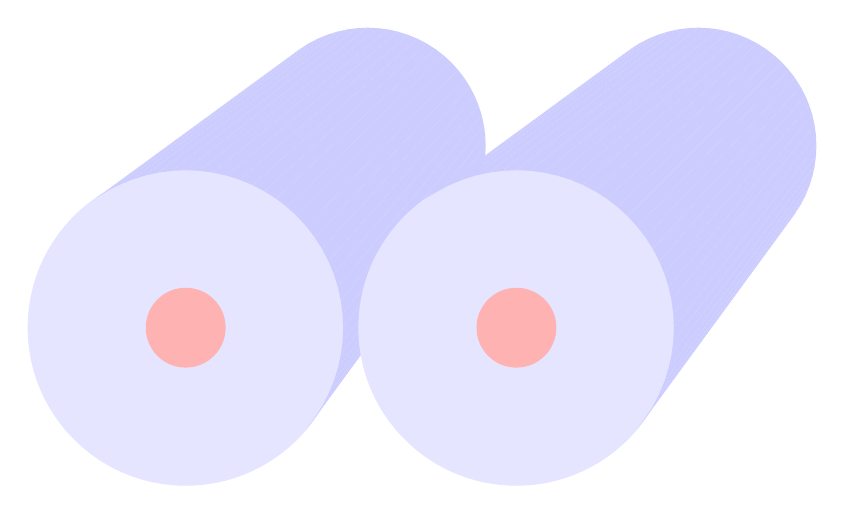
\begin{tikzpicture}[scale=0.5]
    \def\R{4} % Outer radius
    \def\Rb{3} % Outer radius
    \def\r{1} % Inner radius
    \def\L{6} % Half Length of the tube
    \def\S{4.2} % half Shift distance between tubes
    \def\I{5} % increment

    % Left tube
    \draw[blue!10,fill] (-\S,0,\L) circle (\R);   
    \draw[red!30,fill] (-\S,0,\L) circle (\r);    
    %\draw[decorate,decoration=zigzag] (-\S,0,-\L) circle (\Rb);
    \foreach \t in {-40,-35,...,123} {
        \fill[blue!20] ({\R*cos(\t+\I)-\S}, {\R*sin(\t+\I)}, \L) -- ({\R*cos(\t)-\S}, {\R*sin(\t)}, \L) 
        -- ({\Rb*cos(\t)-\S}, {\Rb*sin(\t)}, -\L) -- ({\Rb*cos(\t+\I)-\S}, {\Rb*sin(\t+\I)}, -\L) -- cycle;
    }

    % Right tube    
    \draw[blue!10,fill] (\S,0,\L) circle (\R);   
    \draw[red!30,fill] (\S,0,\L) circle (\r);    
    %\draw[black!10] (\S,0,-\L) circle (\Rb);
    \foreach \t in {-40,-35,...,123} {
        \fill[blue!20] ({\R*cos(\t+\I)+\S}, {\R*sin(\t+\I)}, \L) -- ({\R*cos(\t)+\S}, {\R*sin(\t)}, \L) 
        -- ({\Rb*cos(\t)+\S}, {\Rb*sin(\t)}, -\L) -- ({\Rb*cos(\t+\I)+\S}, {\Rb*sin(\t+\I)}, -\L) -- cycle;
    }
\end{tikzpicture}

%\label{QAM}
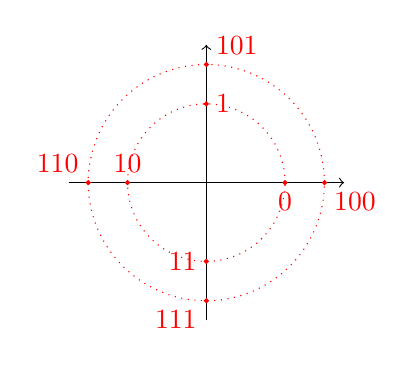
\begin{tikzpicture}[scale=0.5]
    \draw[->] (-3.5,0) -- (3.5, 0);
    \draw[->] (0,-3.5) -- (0,3.5);
    \draw[dotted, red] (0,0) circle(2cm);
    \draw[dotted, red] (0,0) circle(3cm);
    \draw[red, fill] (2,0) circle(0.05cm) node[below] {0};
    \draw[red, fill] (0,2) circle(0.05cm) node[right] {1};
    \draw[red, fill] (-2,0) circle(0.05cm) node[above] {10};
    \draw[red, fill] (0,-2) circle(0.05cm) node[left] {11};
    \draw[red, fill] (3,0) circle(0.05cm) node[below right] {100};
    \draw[red, fill] (0,3) circle(0.05cm) node[above right] {101};
    \draw[red, fill] (-3,0) circle(0.05cm) node[above left] {110};
    \draw[red, fill] (0,-3) circle(0.05cm) node[below left] {111};
\end{tikzpicture}

%\label{8QAM}
\begin{tikzpicture}
    \draw[->] (-3.5,0) -- (3.5, 0);
    \draw[->] (0,-3.5) -- (0,3.5);
    \draw[dashed] (2.5,2.5) -- (-2.5,-2.5);
    \draw[dashed] (-2.5,2.5) -- (2.5,-2.5);
    \draw[dotted, red] (0,0) circle(2cm);
    \draw[dotted, red] (0,0) circle(3cm);
    \draw[red, fill] (45:2) circle(0.05cm) node[above left] {11};
    \draw[red, fill] (135:2) circle(0.05cm) node[above right] {01};
    \draw[red, fill] (225:2) circle(0.05cm) node[above left] {00};
    \draw[red, fill] (-45:2) circle(0.05cm) node[above right] {10};
    \draw[red, fill] (45:3) circle(0.05cm) node[right] {111};
    \draw[red, fill] (135:3) circle(0.05cm) node[left] {101};
    \draw[red, fill] (225:3) circle(0.05cm) node[left] {100};
    \draw[red, fill] (-45:3) circle(0.05cm) node[right] {110};
\end{tikzpicture}

%\label{Bloch-alt}
\tdplotsetmaincoords{0}{0}
\begin{tikzpicture} %[scale=2,tdplot_main_coords]
 \def\rvec{3}
 \def\thetavec{50}
 \def\phivec{40}
 
    %Axes
    \coordinate (O) at (0,0,0);
    \draw[dashed, ->] (0,0,0) -- ++(3.5, 0,0) node[below,right] (x) {x};
    \draw[dashed, ->] (0,-3.5,0) -- ++(0, 7, 0) node[above,right] (y) {y};
    \draw[dashed, ->] (0,0,0) -- ++(0, 0, 3.9) node[below] (z) {$\omega t$};
    \draw[] (0,-3) arc(-90:90:3 and 3);
    \draw[] (0,3) arc (90:270:1.3 and 3);
    \draw[] (-1.2,-1.2) arc (-113:0:3 and 1.35);
    \draw[] (3,0,0) -- ++(0.5, 0, 0);
    \draw[] (0,-3.5,0) -- ++(0, 0.5, 0);
    \draw[] (0,3,0) -- ++(0, 0.5, 0);
    \draw[] (0,0,3) -- ++(0, 0, 0.5);

    % Vector
    \tdplotsetcoord{P}{\rvec}{\thetavec}{\phivec}
    \draw[red,fill] (P) circle(0.05);
    \draw[dashed, red] (O) -- (P) node[circle] (Ptheta) {};
    \draw[dashed, red] (O) -- (Pyz) node[circle] (Pphi) {};
    \draw[dashed, red] (P) -- (Pyz);
    %\draw[dashed, red] (Px) -- (Pxz);

    % angles;
    \draw [shift={(0,0)}, lightgray, fill, fill opacity=0.1] (0,0) -- (P) arc (35:0:1.2) -- cycle;
    \draw [shift={(0,0)}, lightgray, fill, fill opacity=0.1] (0,0) -- (Pyz) arc [start angle=125, delta angle=-12, radius=3.9 ] -- cycle;
    %\draw [shift={(0,0)}, lightgray, fill, fill opacity=0.1] (0,0) -- (Pyz) arc (75:60:1.2) -- cycle;
    \draw( -0.8, 1.6) node[anchor=north west] {$\varphi$};
    \draw( 1.3, 0.8) node[anchor=north west] {$\theta$};
\end{tikzpicture}

%\label{Bloch}
\tdplotsetmaincoords{0}{0}
\begin{tikzpicture} %[scale=2,tdplot_main_coords]
 \def\rvec{3}
 \def\thetavec{70}
 \def\phivec{60}
 
    %Axes
    \coordinate (O) at (0,0,0);
    \draw[->] (0,0,0) -- ++(3.5, 0,0) node[below,right] (y) {y};
    \draw[->] (0,0,0) -- ++(0, 3.5, 0) node[above,right] (z) {z};
    \draw[->] (0,0,0) -- ++(0, 0, 3.5) node[below] (x) {x};
    \draw[] (0,0) circle(3);
    \draw[orange] (-3,0) arc (180:360:3 and 1);
    \draw[dashed, orange] (3,0) arc (0:180:3 and 1);

    % Vector
    \tdplotsetcoord{P}{\rvec}{\thetavec}{\phivec}
    \draw[red,fill] (P) circle(0.05);
    \draw[dashed, red] (O) -- (P) node[circle] (Ptheta) {};
    \draw[dashed, red] (O) -- (Pxz) node[circle] (Pphi) {};
    \draw[dashed, red] (P) -- (Pxz);
    %\draw[dashed, red] (Px) -- (Pxz);

    % angles;
    \draw [shift={(0,0)}, lightgray, fill, fill opacity=0.1] (0,0) -- (65:0.8) arc (65:90:0.8) -- cycle;
    \draw [shift={(0,0)}, lightgray, fill, fill opacity=0.1] (0,0) -- (-135.7:0.6) arc (-135.7:-25:0.6) -- cycle;
    \draw( -0.1, -0.6) node[anchor=north west] {$\varphi$};
    \draw( 0.05, 1.5) node[anchor=north west] {$\theta_B$};
\end{tikzpicture}

%\label{qQPSK}
\begin{tikzpicture}
    \draw[->] (-3.5,0) -- (3.5, 0);
    \draw[->] (0,-3.5) -- (0,3.5);
    \draw[dashed] (2.5,2.5) -- (0,0);
    \draw[dashed] (0,0) -- (2.5,-2.5);
    \draw[dotted, red] (0,0) circle(3cm);
    \draw[red, fill] (3,0) circle(0.05cm) node[below right] {0};
    \draw[red, fill] (0,3) circle(0.05cm) node[above right] {1};
    \draw[red, fill] (2.12,2.12) circle(0.05cm) node[right] {+};
    \draw[red, fill] (2.12,-2.12) circle(0.05cm) node[below] {-};
    \draw[dashed] (1,0) arc (0:45:1) node[right, pos=0.6]{$\theta=\pi/4$};
\end{tikzpicture}

%\label{Grover}
\begin{tikzpicture}
\coordinate (S) at (30:3);
    \draw[red, fill] (S) circle(0.05cm)  node[right] {$\vec{S}$};
    \draw[->, dashed] (0,0) -- (S);
    \draw[->] (0,0) -- (3, 0) node[below] {$\vec{w_v}$};
    \draw[->] (0,0) -- (0,3) node[right] {$\vec{w}$};
    %\draw[dotted, red] (0,0) circle(3cm);
\end{tikzpicture}

%\label{QPSK}

\begin{tikzpicture}
    \draw[->] (-3.5,0) -- (3.5, 0);
    \draw[->] (0,-3.5) -- (0,3.5);
    \draw[dotted, red] (0,0) circle(3cm);
    \draw[red, fill] (3,0) circle(0.05cm) node[below right] {0};
    \draw[red, fill] (0,3) circle(0.05cm) node[above right] {1};
    \draw[red, fill] (-3,0) circle(0.05cm) node[above left] {10};
    \draw[red, fill] (0,-3) circle(0.05cm) node[below left] {11};
\end{tikzpicture}

%
